% SC4022 --- Chapter 6: Dynamics & Spreading (SIR on Networks) (0->100 ground-up)
\chapter{Dynamics \& Spreading: SIR on Networks}
\label{ch:spreading}
\sloppy

\begin{quote}
\emph{``Ideas, like viruses, ride the links.''} --- Whether a rumour dies out or sweeps the world depends not only on how infectious it is but on the wiring it rides.
\end{quote}

\noindent\fbox{\parbox{\dimexpr\linewidth-2\fboxsep-2\fboxrule}{%
\textbf{From zero: we build here, no epidemiology background needed.} We assume only Ch.~1--2 (graph, degree, spectra) and basic probability. SIR, SIS, and threshold models are introduced by story, then formalised, then simulated.}}
\vspace{0.4em}

\section*{Learning Outcomes}
After this chapter you will be able to:
\begin{enumerate}[label=(L\arabic*)]
    \item define SI, SIS, and SIR models on networks (states, rates, transitions);
    \item derive the epidemic threshold $\lambda_c$ via mean-field and via spectral radius;
    \item simulate SIR on ER, small-world, and scale-free graphs and compare outbreaks;
    \item evaluate immunisation strategies: random, degree-targeted, and betweenness-targeted;
    \item describe threshold/cascade models and opinion dynamics as extensions.
\end{enumerate}

% ============================================================
\section{Compartment Models on Graphs}
\label{sec:compartments}
\paragraph{Intuition.} Each person (node) is in a state: \emph{Susceptible} (healthy, can catch), \emph{Infected} (has it, can spread), \emph{Recovered} (immune, out). In continuous time, an infected node infects each susceptible neighbour at rate $\beta$ and recovers at rate $\mu$. The ratio $\lambda=\beta/\mu$ is the \emph{effective spreading rate}. If $\lambda$ is tiny, the outbreak fizzles; if large, it explodes---where is the boundary?

\begin{definition}[SIR, SIS, SI on networks]\label{def:sir}
States per node: $S\to I\to R$ (SIR, permanent immunity), $S\to I\to S$ (SIS, can be reinfected), $S\to I$ (SI, never recovers). For SIR, let $s_v(t),\,i_v(t),\,r_v(t)$ be probabilities node $v$ is in each state ($s+i+r=1$). Mean-field (quenched) dynamics:
\begin{equation}
\dot i_v=\beta s_v\sum_u A_{vu}i_u-\mu i_v,\quad \dot s_v=-\beta s_v\sum_u A_{vu}i_u,\quad \dot r_v=\mu i_v.
\end{equation}
SIS drops the $R$ equation and adds $+\mu i_v$ to $\dot s_v$. SI sets $\mu=0$.
\end{definition}

\begin{figure}[h]\centering
\begin{tikzpicture}[scale=0.82,every node/.style={font=\scriptsize}]
% compartments
\node[draw,thick,fill=blue!14,rounded corners=4pt,minimum width=2.0cm,minimum height=1.0cm,align=center] (S) at (0,1.0) {\textbf{S}\\\tiny susceptible};
\node[draw,thick,fill=red!14,rounded corners=4pt,minimum width=2.0cm,minimum height=1.0cm,align=center] (I) at (3.5,1.0) {\textbf{I}\\\tiny infected};
\node[draw,thick,fill=green!14,rounded corners=4pt,minimum width=2.0cm,minimum height=1.0cm,align=center] (R) at (7.0,1.0) {\textbf{R}\\\tiny recovered};
\draw[->,thick,blue!60!black] (S)--(I) node[midway,above,font=\tiny,fill=yellow!10,rounded corners=2pt,inner sep=2pt] {$\beta$ per SI edge};
\draw[->,thick,orange!70!black] (I)--(R) node[midway,above,font=\tiny,fill=yellow!10,rounded corners=2pt,inner sep=2pt] {$\mu$ recovery};
\draw[->,thick,green!50!black,dashed,rounded corners=4pt] (R.south) -- ++(0,-0.7) -- ++(-3.5,0) -- (S.south) node[midway,below,font=\tiny,fill=green!10,rounded corners=2pt,inner sep=2pt] {SIS: $R\to S$ (reinfect)};
% star outbreak illustration below
\begin{scope}[yshift=-2.0cm]
\node[circle,draw,thick,fill=red!18,minimum size=0.7cm] (hub) at (1.5,0.6) {I};
\foreach \a/\st in {30/blue!12,90/blue!12,150/red!10,210/blue!12,330/blue!12} {
\node[circle,draw,thick,fill=\st,minimum size=0.55cm] at ($(hub)+(\a:1.15)$) {\tiny S};}
\foreach \a in {30,90,150,210,330} \draw[thick] (hub)--($(hub)+(\a:1.15)$);
\node[font=\tiny,fill=red!10,rounded corners=2pt,inner sep=2pt] at (1.5,-0.85) {hub infects many};
\end{scope}
\begin{scope}[xshift=5.0cm,yshift=-2.0cm]
\node[circle,draw,thick,fill=blue!12,minimum size=0.6cm] (a) at (0,0.6) {S};
\node[circle,draw,thick,fill=blue!12,minimum size=0.6cm] (b) at (1.4,0.6) {S};
\node[circle,draw,thick,fill=blue!12,minimum size=0.6cm] (c) at (2.8,0.6) {S};
\draw[thick] (a)--(b)--(c);
\node[font=\tiny,fill=blue!10,rounded corners=2pt,inner sep=2pt] at (1.4,-0.85) {chain: slow spread};
\end{scope}
\node[font=\tiny,draw=gray!40,fill=yellow!8,rounded corners=2pt,inner sep=3pt] at (3.5,-3.3) {\textcolor{blue!60!black}{$\blacksquare$ S} \quad \textcolor{red!60!black}{$\blacksquare$ I} \quad \textcolor{green!50!black}{$\blacksquare$ R} \quad \textcolor{orange!70!black}{$\blacksquare$ hub accelerates}};
\end{tikzpicture}
\caption{Compartment models and why hubs matter. Top: $S\to I$ at rate $\beta$ per SI edge, $I\to R$ at $\mu$; dashed is SIS reinfection. Bottom: a star hub reaches many susceptibles at once (fast), a chain spreads one hop at a time (slow).}
\label{fig:sir-compartments}
\end{figure}

% ============================================================
\section{Epidemic Threshold}
\label{sec:threshold}
\paragraph{Intuition.} If each infected node on average infects less than one new node before recovering, the outbreak shrinks; if more than one, it grows. On a network, ``average'' depends on who you are connected to---hubs amplify, leaves dampen. The tipping point is an eigenvalue.

\begin{theorem}[Spectral threshold for SIS/SIR]\label{thm:threshold}
For the quenched mean-field model with adjacency $A$ and spectral radius $\rho(A)=\lambda_{\max}(A)$,
\begin{equation}
\lambda_c=\frac{\beta}{\mu}\Big|_{\text{crit}}=\frac1{\rho(A)}.
\end{equation}
If $\lambda<\lambda_c$, the disease-free state is stable (outbreak dies); if $\lambda>\lambda_c$, endemic/explosive spread occurs. For annealed (degree-based) mean-field,
$\lambda_c^{\text{HMF}}=\langle k\rangle/\langle k^2\rangle$.
\end{theorem}
\begin{proof}[Idea]
Linearise around disease-free ($s_v\approx1$, $i_v\approx0$): $\dot i = (\beta A-\mu I)i$. Growth is governed by the largest eigenvalue of $\beta A-\mu I$, namely $\beta\rho(A)-\mu$. It turns positive exactly when $\beta/\mu>1/\rho(A)$. Heterogeneous mean-field averages over degree classes to get $\langle k^2\rangle/\langle k\rangle$. \qed
\end{proof}

Consequences tie directly to Ch.~5: for scale-free $P(k)\sim k^{-\gamma}$ with $2<\gamma<3$, $\langle k^2\rangle$ diverges, so $\lambda_c^{\text{HMF}}\to0$ as $n\to\infty$---arbitrarily weak viruses persist (no threshold in the infinite limit). ER graphs have finite $\langle k^2\rangle$, so a genuine threshold remains.

\begin{figure}[h]\centering
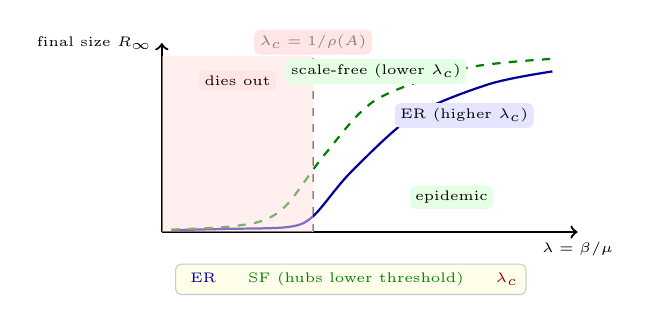
\begin{tikzpicture}[scale=0.80,every node/.style={font=\scriptsize}]
\draw[->,thick] (0,0)--(6.6,0) node[below,font=\tiny] {$\lambda=\beta/\mu$};
\draw[->,thick] (0,0)--(0,3.0) node[left,font=\tiny] {final size $R_\infty$};
\draw[dashed,gray,thick] (2.4,0)--(2.4,2.8) node[above,font=\tiny,fill=red!10,rounded corners=2pt,inner sep=2pt] {$\lambda_c=1/\rho(A)$};
\draw[thick,blue!60!black,smooth] plot coordinates {(0.15,0.03) (1.0,0.05) (2.0,0.08) (2.4,0.25) (3.0,0.95) (4.0,1.85) (5.2,2.35) (6.2,2.55)};
\draw[thick,green!50!black,dashed,smooth] plot coordinates {(0.15,0.04) (1.0,0.08) (1.6,0.18) (2.0,0.45) (2.6,1.25) (3.4,2.10) (4.8,2.60) (6.2,2.75)};
\fill[red!12,opacity=0.5] (0,0) rectangle (2.4,2.8);
\node[font=\tiny,fill=red!10,rounded corners=2pt,inner sep=2pt] at (1.2,2.4) {dies out};
\node[font=\tiny,fill=green!10,rounded corners=2pt,inner sep=2pt] at (4.6,0.55) {epidemic};
\node[font=\tiny,fill=blue!10,rounded corners=2pt,inner sep=2pt] at (4.8,1.85) {ER (higher $\lambda_c$)};
\node[font=\tiny,fill=green!10,rounded corners=2pt,inner sep=2pt] at (3.4,2.55) {scale-free (lower $\lambda_c$)};
\node[font=\tiny,draw=gray!40,fill=yellow!8,rounded corners=2pt,inner sep=3pt] at (3.0,-0.75) {\textcolor{blue!60!black}{$\blacksquare$ ER} \quad \textcolor{green!50!black}{$\blacksquare$ SF (hubs lower threshold)} \quad \textcolor{red!60!black}{$\blacksquare$ $\lambda_c$}};
\end{tikzpicture}
\caption{Epidemic threshold. Below $\lambda_c$ final recovered fraction is near zero; above it jumps. Scale-free networks (green, hubs) have smaller $\lambda_c$ than ER (blue) of same $\langle k\rangle$ because $\rho(A)$ is larger when hubs exist.}
\label{fig:threshold}
\end{figure}

\begin{figure}[h]\centering
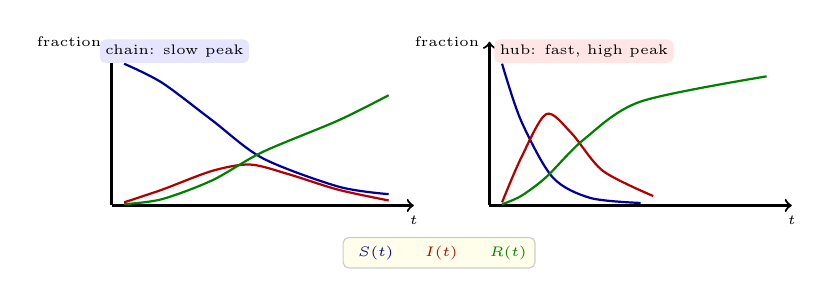
\begin{tikzpicture}[scale=0.80,every node/.style={font=\scriptsize}]
% SIR time series on chain vs hub
\draw[->,thick] (0,0)--(4.8,0) node[below,font=\tiny] {$t$};
\draw[->,thick] (0,0)--(0,2.6) node[left,font=\tiny] {fraction};
% chain SIR: slow, low peak
\draw[thick,blue!60!black,smooth] plot coordinates {(0.2,2.25) (0.8,1.95) (1.6,1.35) (2.4,0.75) (3.6,0.30) (4.4,0.18)};
\draw[thick,red!70!black,smooth] plot coordinates {(0.2,0.05) (0.8,0.25) (1.6,0.55) (2.2,0.65) (2.8,0.50) (3.6,0.25) (4.4,0.08)};
\draw[thick,green!50!black,smooth] plot coordinates {(0.2,0.02) (0.8,0.10) (1.6,0.40) (2.4,0.85) (3.6,1.35) (4.4,1.75)};
\node[font=\tiny,fill=blue!10,rounded corners=2pt,inner sep=2pt] at (1.0,2.45) {chain: slow peak};
% hub SIR on right
\begin{scope}[xshift=6.0cm]
\draw[->,thick] (0,0)--(4.8,0) node[below,font=\tiny] {$t$};
\draw[->,thick] (0,0)--(0,2.6) node[left,font=\tiny] {fraction};
\draw[thick,blue!60!black,smooth] plot coordinates {(0.2,2.25) (0.5,1.35) (1.0,0.45) (1.6,0.12) (2.4,0.04)};
\draw[thick,red!70!black,smooth] plot coordinates {(0.2,0.05) (0.5,0.75) (0.9,1.45) (1.3,1.15) (1.8,0.55) (2.6,0.15)};
\draw[thick,green!50!black,smooth] plot coordinates {(0.2,0.02) (0.5,0.15) (0.9,0.45) (1.5,1.05) (2.4,1.65) (4.4,2.05)};
\node[font=\tiny,fill=red!10,rounded corners=2pt,inner sep=2pt] at (1.5,2.45) {hub: fast, high peak};
\end{scope}
\node[font=\tiny,draw=gray!40,fill=yellow!8,rounded corners=2pt,inner sep=3pt] at (5.2,-0.75) {\textcolor{blue!60!black}{$\blacksquare$ $S(t)$} \quad \textcolor{red!70!black}{$\blacksquare$ $I(t)$} \quad \textcolor{green!50!black}{$\blacksquare$ $R(t)$}};
\end{tikzpicture}
\caption{SIR curves $S(t),I(t),R(t)$ on a chain (left: broad, low peak) vs a star-like network (right: sharp, high peak). Hubs synchronise infections---the epidemic is faster and larger.}
\label{fig:sir-curves}
\end{figure}

% ============================================================
\section{Immunisation and Influence}
\label{sec:immunisation}
\paragraph{Intuition.} Vaccinating a random person protects one node; vaccinating a hub protects many paths. To stop an outbreak cheaply, target high-degree or high-betweenness nodes (acquaintance immunisation picks a random neighbour---biased toward hubs---when global ranking is unknown). The same logic flipped is \emph{influence maximisation}: seed the best spreaders to maximise adoption.

\begin{lstlisting}[language=Python, caption={SIR simulation on ER vs BA: threshold and final size.}, label={lst:sir-sim}]
import networkx as nx
import numpy as np

def sir_final_size(G, beta=0.3, mu=0.2, seed=0):
    # Simple discrete-time SIR (parallel update)
    import random; random.seed(seed)
    infected = {next(iter(G.nodes()))}
    recovered = set(); susceptible = set(G.nodes()) - infected
    while infected:
        new_inf = set()
        for v in list(infected):
            for nb in G.neighbors(v):
                if nb in susceptible and random.random() < beta:
                    new_inf.add(nb)
            if random.random() < mu:
                recovered.add(v); infected.remove(v)
        susceptible -= new_inf; infected |= new_inf
        if len(recovered) > 5*G.number_of_nodes(): break
    return len(recovered) / G.number_of_nodes()

for name, G in [("ER", nx.erdos_renyi_graph(200,0.03,seed=1)),
                ("BA", nx.barabasi_albert_graph(200,3,seed=1))]:
    rho = max(np.linalg.eigvals(nx.to_numpy_array(G)).real)
    print(name, f"rho={rho:.1f} lambda_c~{1/rho:.3f}"
          f" final R={sir_final_size(G,beta=0.25,mu=0.2):.2f}")
\end{lstlisting}

\begin{lstlisting}[language=Python, caption={Targeted vs random immunisation: removing hubs collapses spreading.}, label={lst:immunisation}]
import networkx as nx

def giant_after_removal(G, remove):
    H = G.copy(); H.remove_nodes_from(remove)
    if not H: return 0
    return max(len(c) for c in nx.connected_components(H)) / G.number_of_nodes()

G = nx.barabasi_albert_graph(200, 3, seed=0)
# Random vs degree-targeted removal of 10 nodes
import random; random.seed(0)
rand10 = random.sample(list(G.nodes()), 10)
hub10 = sorted(G.degree, key=lambda x: x[1], reverse=True)[:10]
hub10 = [v for v,_ in hub10]
print(f"random 10 removal: giant={giant_after_removal(G, rand10):.2f}")
print(f"hub 10 removal:    giant={giant_after_removal(G, hub10):.2f}")
# Hub removal shatters scale-free networks (Ch.7 preview)
\end{lstlisting}

% ============================================================
\section{Beyond SIR: Thresholds, Cascades, Opinions}
\label{sec:beyond-sir}
Not all spreading is simple contagion (one contact can infect). In \emph{complex contagion} a node adopts only when a fraction $\phi$ of neighbours have adopted---capturing social reinforcement. The \emph{linear threshold} and \emph{independent cascade} models formalise this; influence maximisation becomes NP-hard but greedy gives a $(1-1/e)$ approximation (submodularity). Opinion dynamics (voter, DeGroot) add continuous states. All run on the same wiring---topology still governs speed and reach.

% ============================================================
\section{Chapter Notes}
Kermack and McKendrick (1927) founded compartmental epidemics; Pastor-Satorras and Vespignani (2001) linked the threshold to $\langle k^2\rangle/\langle k\rangle$ on scale-free nets; Chakrabarti et~al.\ (2008) gave the spectral form $\lambda_c=1/\rho(A)$. Discrete-time SIR used in code follows the Gillespie / synchronous update family. Immunisation surveys: Pastor-Satorras et~al.\ (2015). For influence maximisation, Kempe--Kleinberg--Tardos (2003) is the landmark.

% ============================================================
\section{Exercises}
\label{sec:ch06-exercises}
\begin{enumerate}[label=E6.\arabic*, leftmargin=*, itemsep=0.8em]
    \item \textbf{SI on a star.} Consider SI ($\mu=0$) on a star with centre $1$ and leaves $2,\dots,n$. Start with centre infected. Derive expected time to infect all leaves if each SI edge transmits with probability $\beta$ per step (discrete time, independent).
    \item \textbf{Threshold comparison.} For ER with $n=500$, $p=0.01$ and BA with $n=500$, $m=3$ (same $\langle k\rangle\approx6$), estimate $\rho(A)$ numerically and predict $\lambda_c$. Simulate SIR at $\lambda=0.8\lambda_c$ and $1.2\lambda_c$ and compare final sizes.
    \item \textbf{Mean-field vs spectral.} Compute $\langle k\rangle$, $\langle k^2\rangle$, and $\rho(A)$ for a 100-node BA graph. Compare $\lambda_c^{\text{HMF}}=\langle k\rangle/\langle k^2\rangle$ vs $1/\rho(A)$. Which is smaller? Why does HMF underestimate the threshold on clustered graphs?
    \item \textbf{Immunisation sweep.} On BA(200,3), remove nodes in random order vs degree-descending order (5 at a time, up to 40). Plot giant-component fraction vs number removed. At what removal fraction does targeted attack halve the giant?
    \item \textbf{Complex contagion.} Simulate linear-threshold with $\phi=0.4$ on a 30-node WS graph ($k=4$, $p=0.1$). Seed two adjacent vs two distant nodes and report final adoption. Why does clustering help complex but hinder simple contagion?
\end{enumerate}
% End of Chapter 6
